\subsection*{Problema 26}

\noindent\textbf{Enunciado:} \\
Calcular la integral indefinida:
\begin{align*}
I = \int \dfrac{dx}{1 + \sin^2 x}
\end{align*}

\noindent\textbf{Solución:} \\
Siguiendo las indicaciones, dividimos tanto el numerador como el denominador por $\cos^2 x$:
\begin{align*}
I &= \int \dfrac{\dfrac{1}{\cos^2 x} dx}{\dfrac{1}{\cos^2 x} + \dfrac{\sin^2 x}{\cos^2 x}} \\
I &= \int \dfrac{\sec^2 x \, dx}{\sec^2 x + \tan^2 x}
\end{align*}

Utilizamos la identidad trigonométrica fundamental $\sec^2 x = 1 + \tan^2 x$ en el denominador:
\begin{align*}
I &= \int \dfrac{\sec^2 x \, dx}{(1 + \tan^2 x) + \tan^2 x} \\
I &= \int \dfrac{\sec^2 x \, dx}{1 + 2\tan^2 x}
\end{align*}

Aplicamos el método de sustitución. Sea $u = \tan x$, entonces su diferencial es:
\begin{align*}
du = \sec^2 x \, dx
\end{align*}

Sustituyendo en la integral, obtenemos una forma estándar de arcotangente:
\begin{align*}
I &= \int \dfrac{du}{1 + (\sqrt{2}u)^2}
\end{align*}

Aplicando la fórmula de integración $\int \dfrac{du}{1 + a^2 u^2} = \dfrac{1}{a}\arctan(au) + C$:
\begin{align*}
I &= \dfrac{1}{\sqrt{2}} \arctan(\sqrt{2}u) + C
\end{align*}

Regresando a la variable original $x$ mediante $u = \tan x$:
\begin{align*}
I &= \dfrac{1}{\sqrt{2}} \arctan(\sqrt{2}\tan x) + C
\end{align*}

Por lo tanto, el resultado de la integral es:
\begin{align*}
\int \dfrac{dx}{1 + \sin^2 x} = \dfrac{\sqrt{2}}{2} \arctan(\sqrt{2}\tan x) + C
\end{align*}

\begin{figure}[H]
	\centering
	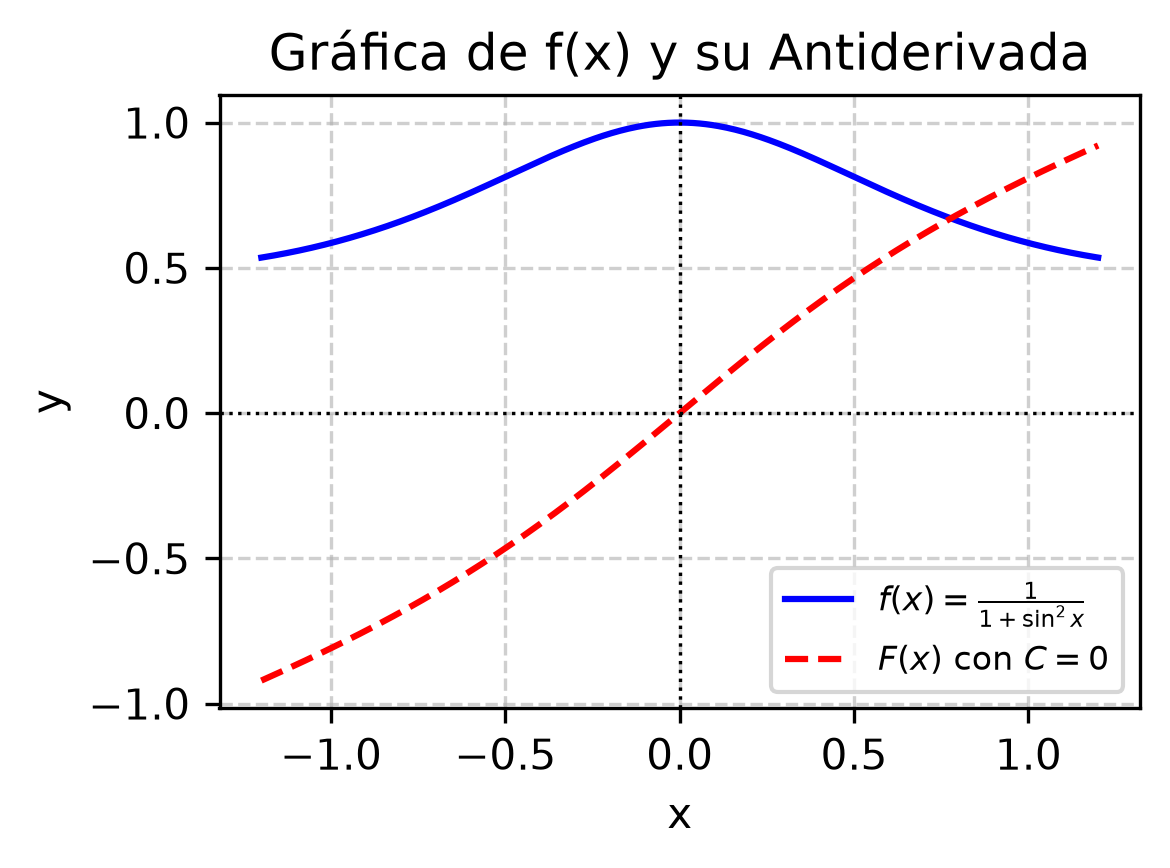
\includegraphics[width=\columnwidth]{semana_04/graficas/SEM04_P26_grafica.png}
	\caption{Representación gráfica de $f(x)$ y su antiderivada $F(x)$ evaluada para la constante de integración $C = 0$ (Problema 26).}
	\label{fig:problema26}
\end{figure}
